% THIS IS AN EXAMPLE DOCUMENT FOR VLDB 2012
% based on ACM SIGPROC-SP.TEX VERSION 2.7
% Modified by  Gerald Weber <gerald@cs.auckland.ac.nz>
% Removed the requirement to include *bbl file in here. (AhmetSacan, Sep2012)
% Fixed the equation on page 3 to prevent line overflow. (AhmetSacan, Sep2012)

\documentclass{vldb}
\usepackage{graphicx}
\usepackage{xspace}
\usepackage{balance}  % for  \balance command ON LAST PAGE  (only there!)

\newcommand{\probkb}{\textsc{ProbKB}\xspace}
\newcommand{\nell}{\textsc{Nell}\xspace}

\begin{document}

% ****************** TITLE ****************************************

\title{ProbKB: Managing Evolving Web Knowledge}

% possible, but not really needed or used for PVLDB:
%\subtitle{[Extended Abstract]
%\titlenote{A full version of this paper is available as\textit{Author's Guide to Preparing ACM SIG Proceedings Using \LaTeX$2_\epsilon$\ and BibTeX} at \texttt{www.acm.org/eaddress.htm}}}

% ****************** AUTHORS **************************************

% You need the command \numberofauthors to handle the 'placement
% and alignment' of the authors beneath the title.
%
% For aesthetic reasons, we recommend 'three authors at a time'
% i.e. three 'name/affiliation blocks' be placed beneath the title.
%
% NOTE: You are NOT restricted in how many 'rows' of
% "name/affiliations" may appear. We just ask that you restrict
% the number of 'columns' to three.
%
% Because of the available 'opening page real-estate'
% we ask you to refrain from putting more than six authors
% (two rows with three columns) beneath the article title.
% More than six makes the first-page appear very cluttered indeed.
%
% Use the \alignauthor commands to handle the names
% and affiliations for an 'aesthetic maximum' of six authors.
% Add names, affiliations, addresses for
% the seventh etc. author(s) as the argument for the
% \additionalauthors command.
% These 'additional authors' will be output/set for you
% without further effort on your part as the last section in
% the body of your article BEFORE References or any Appendices.

\numberofauthors{2} %  in this sample file, there are a *total*
% of EIGHT authors. SIX appear on the 'first-page' (for formatting
% reasons) and the remaining two appear in the \additionalauthors section.

\author{
% You can go ahead and credit any number of authors here,
% e.g. one 'row of three' or two rows (consisting of one row of three
% and a second row of one, two or three).
%
% The command \alignauthor (no curly braces needed) should
% precede each author name, affiliation/snail-mail address and
% e-mail address. Additionally, tag each line of
% affiliation/address with \affaddr, and tag the
% e-mail address with \email.
%
% 1st. author
\alignauthor
Yang Chen\\%\titlenote{Dr.~Trovato insisted his name be first.}\\
       \affaddr{Department of CISE}\\
       \affaddr{University of Florida}\\
       \affaddr{Florida, USA}\\
       \email{yang@cise.ufl.edu}
% 2nd. author
\alignauthor
Daisy Zhe Wang\\%\titlenote{The secretary disavows}
       \affaddr{Department of CISE}\\
       \affaddr{University of Florida}\\
       \affaddr{Florida, USA}\\
       \email{daisyw@cise.ufl.edu}
%\and  % use '\and' if you need 'another row' of 3 author names
}
% There's nothing stopping you putting the seventh, eighth, etc.
% author on the opening page (as the 'third row') but we ask,
% for aesthetic reasons that you place these 'additional authors'
% in the \additional authors block, viz.
\additionalauthors{Additional authors: John Smith (The Th{\o}rv\"{a}ld Group, {\texttt{jsmith@affiliation.org}}), Julius P.~Kumquat
(The \raggedright{Kumquat} Consortium, {\small \texttt{jpkumquat@consortium.net}}), and Ahmet Sacan (Drexel University, {\small \texttt{ahmetdevel@gmail.com}})}
\date{30 July 1999}
% Just remember to make sure that the TOTAL number of authors
% is the number that will appear on the first page PLUS the
% number that will appear in the \additionalauthors section.


\maketitle

\begin{abstract}
Abstract
\end{abstract}

\section{Introduction}

\section{Preliminaries}

\subsection{Markov Logic Networks}

\subsection{Factor Graphs}

\subsection{Metropolis-Hastings}

\section{The {\large{\probkb}} System}
\begin{figure}[ht]
  \centering
  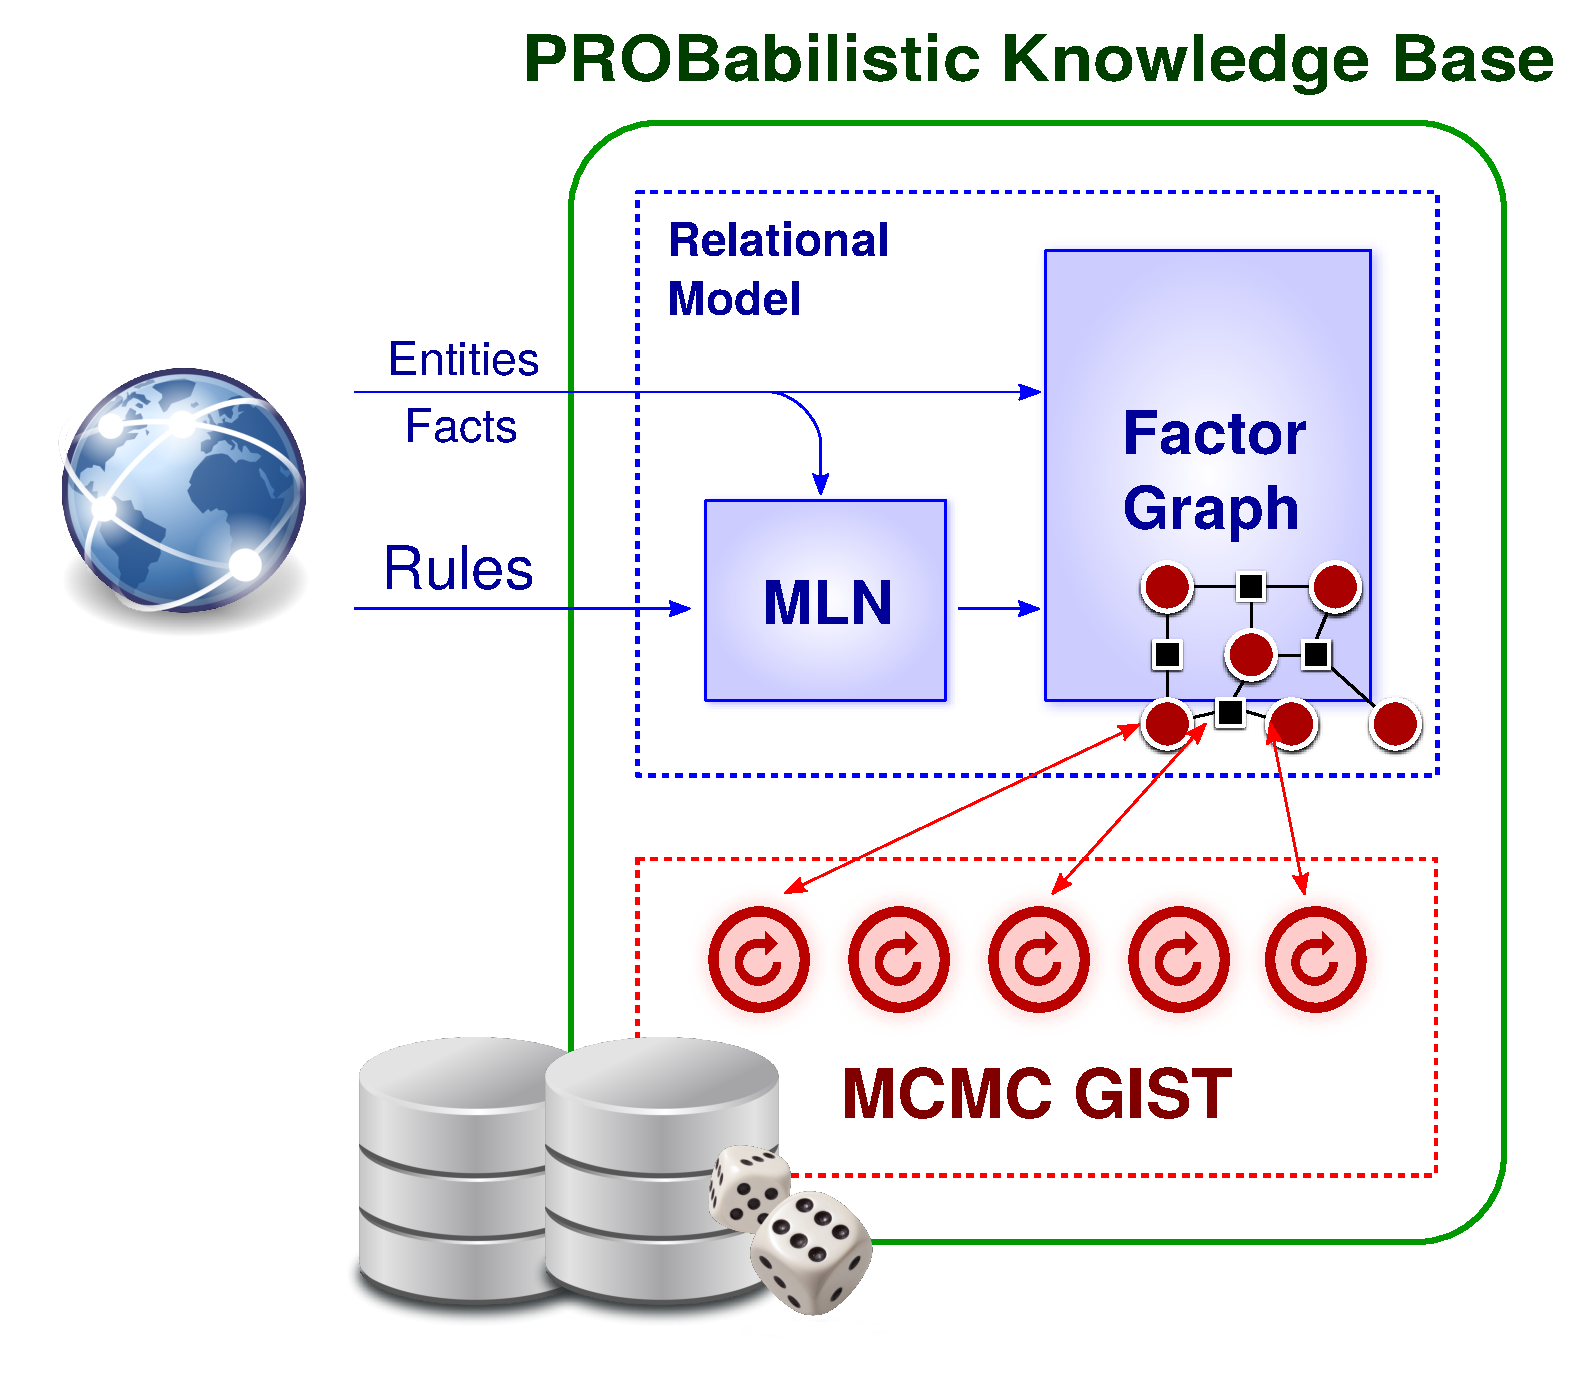
\includegraphics[clip,trim=20 30 0 15,width=.9\columnwidth]{architecture.pdf}
  \caption{\probkb system architecture.}
  \label{fig:architecture}
\end{figure}

\subsection{First-Order Horn Clauses}
In this paper, we focus on first-order Horn clauses only, though in general Markov logic supports arbitrary clauses. This decision is reasonable in our context since we use Markov logic to represent extracted general-purpose rules rather than hand-crafted ones encoding complex algorithms that work in specific domains. As an example of such generality, consider the \nell knowledge base~\cite{}, where we have extracted entities and their relationships. Then our interest would be to know whether a certain fact \texttt{R(x,y)} is likely to hold given these extractions. This is best done by using rules such as $p\leftarrow q_1\ldots q_n$ to infer new facts using existing ones. We are less interested, however, in imposing constraints on the knowledge base using complex rules.

On the contrary, suppose we want to do joint segmentation using Markov logic, then we need more complex rules to specify assumptions and inputs to a specific algorithm. The Markov logic program provided on the Alchemy~\cite{} website shows how we can do it. 

\subsection{The Relational MLN Model}
We restrict our attention to first-order Horn clauses. This greatly simplies the rules we need to consider.

For all rules of the form $$p(x,y)\leftarrow q(x,z), r(z,y),$$ we have a row in a table called $M_3$.

\subsection{Graph Aggregation}
Shared memory?

\subsection{Inference}

\subsection{Incremental Inference}

\section{Experiments}

\subsection{Grounding}


% ensure same length columns on last page (might need two sub-sequent latex runs)
\balance

%ACKNOWLEDGMENTS are optional
\section{Acknowledgments}


% The following two commands are all you need in the
% initial runs of your .tex file to
% produce the bibliography for the citations in your paper.
\bibliographystyle{abbrv}
\bibliography{probkb}  % vldb_sample.bib is the name of the Bibliography in this case
% You must have a proper ".bib" file
%  and remember to run:
% latex bibtex latex latex
% to resolve all references

\section{References}


%APPENDIX is optional.
% ****************** APPENDIX **************************************
% Example of an appendix; typically would start on a new page
%pagebreak

\begin{appendix}
You can use an appendix for optional proofs or details of your evaluation which are not absolutely necessary to the core understanding of your paper. 
\end{appendix}



\end{document}
